\vspace{5mm}

\noindent\parbox{8.3cm}{\parpic{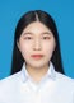
\includegraphics[width=2.84cm]{Yingying Shi.pdf}}{\small\quad {\bf Ying-Ying Shi}  {is now a postgraduate in Shanghai Key Laboratory of Trustworthy Computing and Software Engineering Institute, East China Normal University, Shanghai. Her current research interests include linear temporal logic and automaton. }}\\[1mm]}

\noindent\parbox{8.3cm}{\parpic{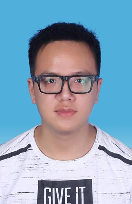
\includegraphics[width=2.84cm]{Shengping Xiao.pdf}}{\small\quad {\bf Sheng-Ping Xiao}  {is an undergraduate student in Shanghai Key Laboratory of Trustworthy Computing and Software Engineering Institute, East China Normal University, Shanghai. His current research interests include logic and automaton. }}\\[1mm]}

\noindent\parbox{8.3cm}{\parpic{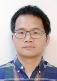
\includegraphics[width=2.84cm]{Jianwen Li.pdf}}{\small\quad {\bf Jian-Wen Li}  {is now a research professor in East China Normal University. He received his Ph.D. from East China Normal University in 2014. His research interests focus on formal method and automatic verification techniques.}}\\[1mm]}

 \noindent\parbox{8.3cm}{\parpic{
\includegraphics[width=2.84cm]{Jian Guo.pdf}}{\small\quad {\bf Jian Guo}  {is an associated professor in the Software Engineering Institute of East China Normal University. she holds her PhD degree in microelectronics from Xidian University, China. Her current research fields are related to model, design and verify operation system, model checking of CTL, LTL.}}\\[1mm]}

\noindent\parbox{8.3cm}{\parpic{
\includegraphics[width=2.84cm]{Geguang Pu.pdf}}{\small\quad {\bf Ge-Guang Pu} is now a full professor in East China Normal University. He recieved his Ph.D. from Peking University in 2007. His research interests focus on software engineering and formal methods.  }\\[1mm]}
